\chapter{Use case}

%begin free user section
\section{Free-user}
	\subsection{General Use Case}
		\begin{figure}[ht]
			\begin{center}
				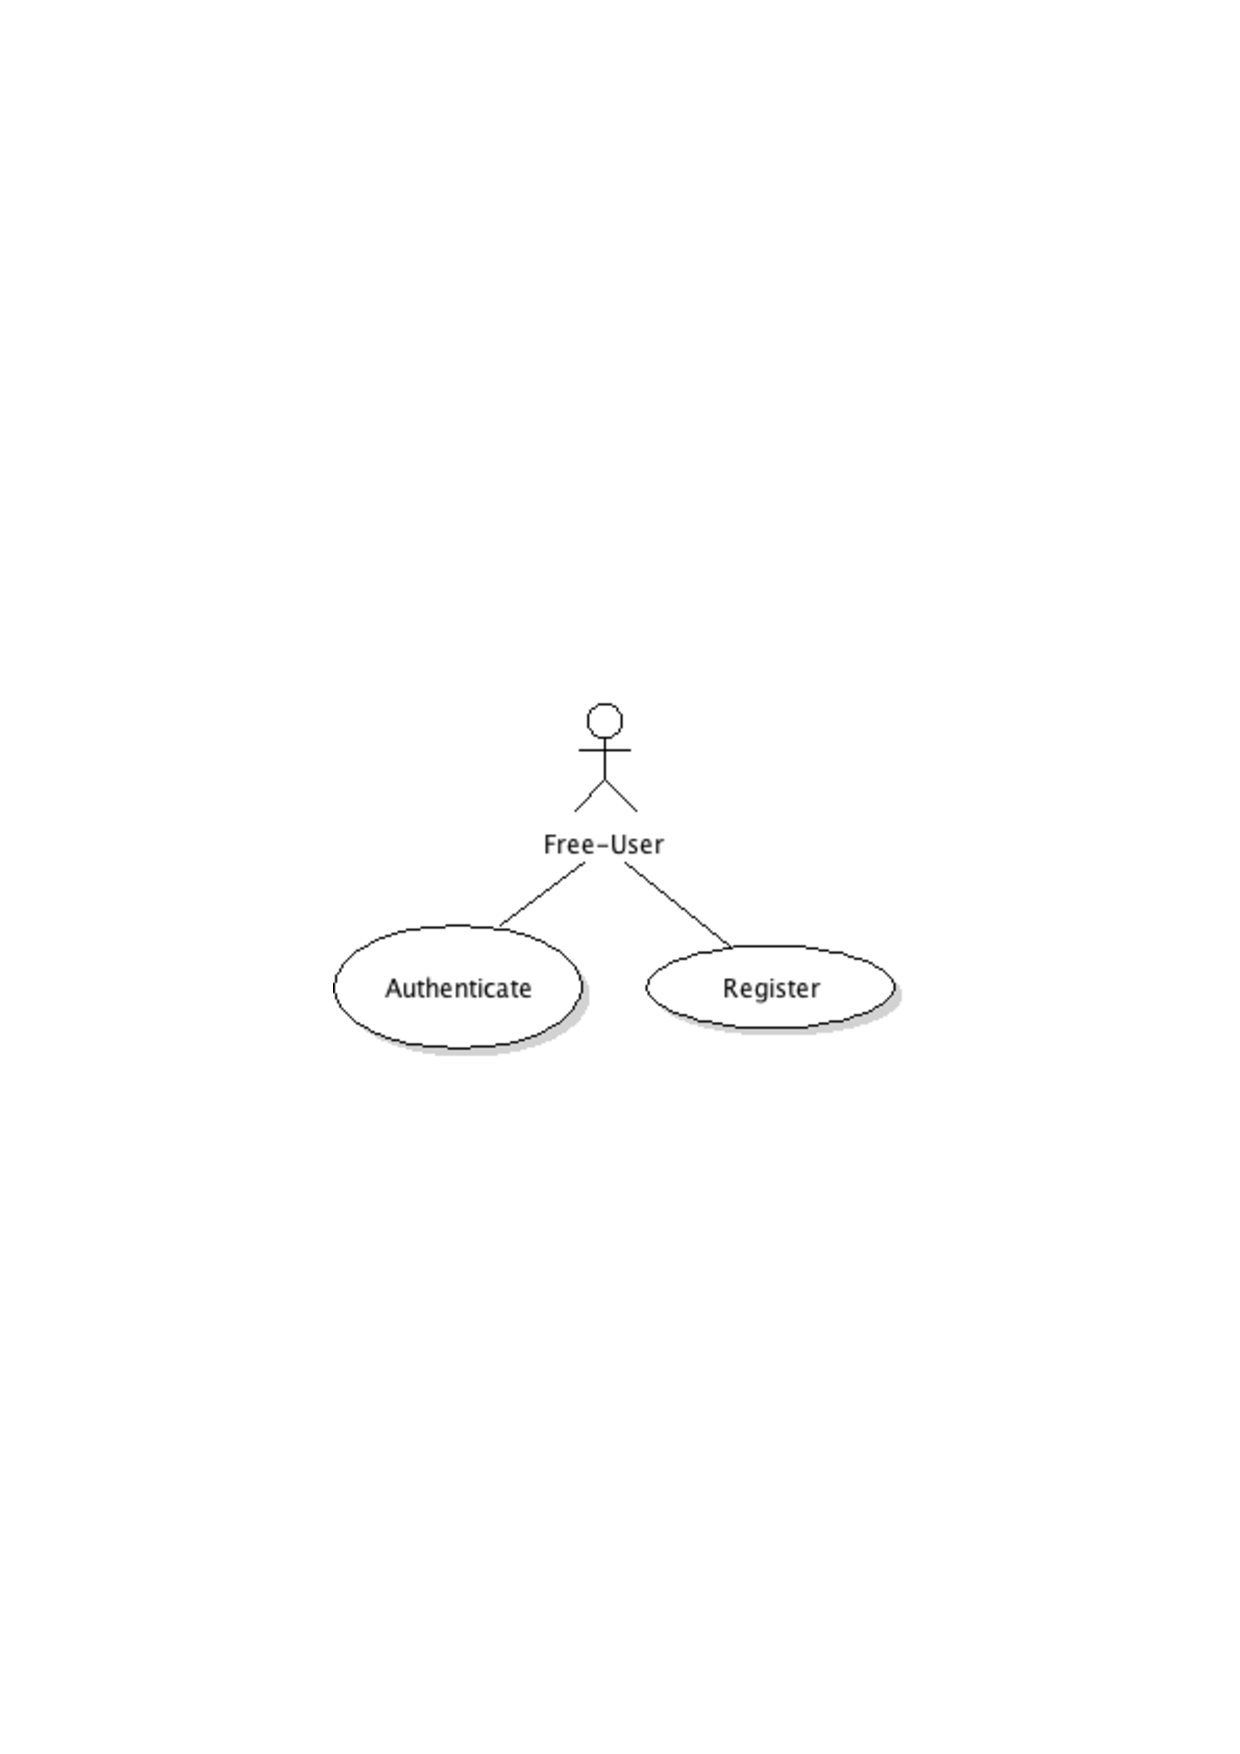
\includegraphics[width=\textwidth,  trim=2cm 10cm 2cm 11cm]{UML_figure/UC/free_user/UC_FreeUser_General.pdf}
				\caption{Free-User Use Case : Overview}
			\end{center}
		\end{figure}
		A free user is a user non identified by the platform. He has the following features~:
	\subsection{Register}Register a free-user to have access to the different features
		Information needed are 
	\subsection{Authenticate}Identify free-user and if registered give him access to the different features
%end free user section
\newpage
%begin student section
\section{Student}
	\subsection{General Use Case}
		\begin{figure}[ht]
			\begin{center}
				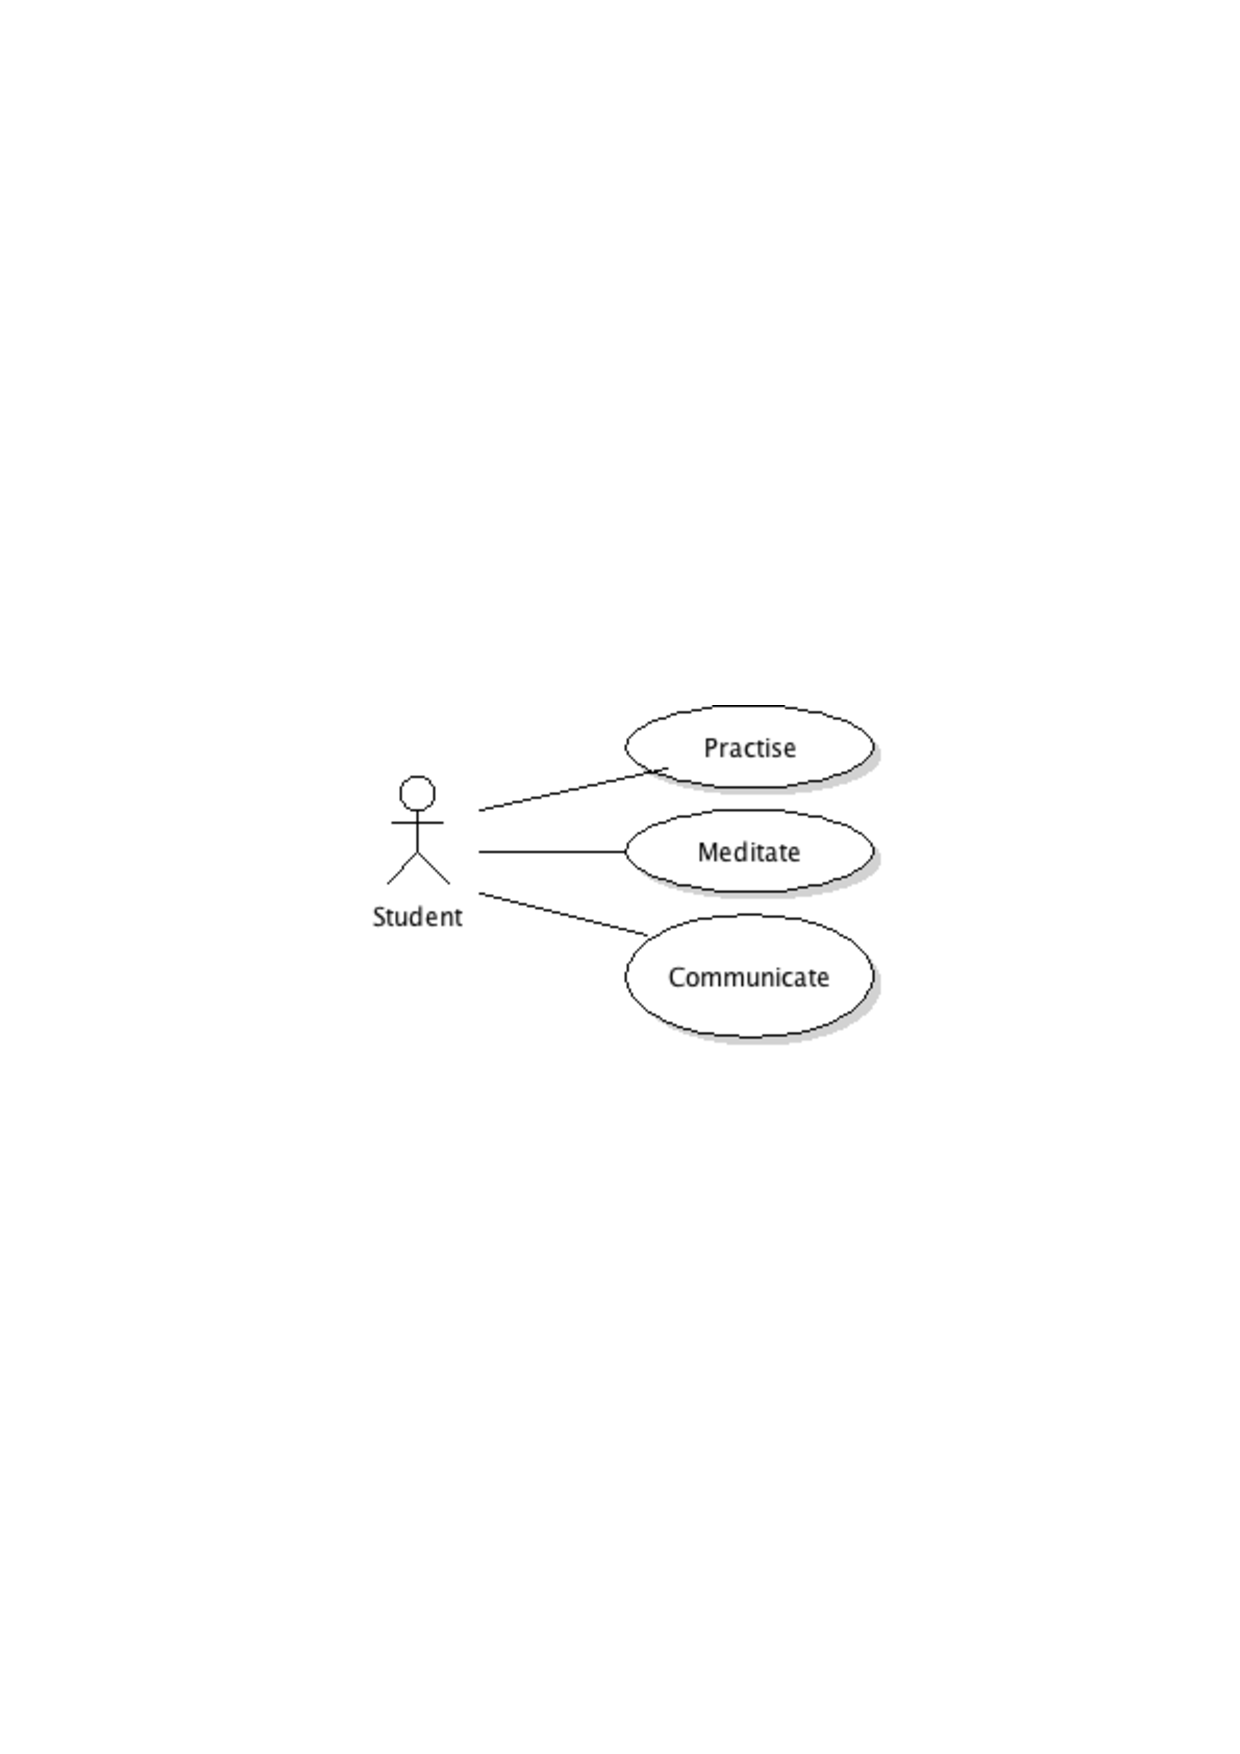
\includegraphics[width=\textwidth,  trim=2cm 10cm 2cm 11cm]{UML_figure/UC/student/UC_Student_General.pdf}
				\caption{Student Use Case : Overview}
			\end{center}
		\end{figure}
		A user identify as a student has three major action which are Practise, Meditate and Communicate.
	\subsection{Practise}
		A student user can train to improve his skills in programming languages. 
		
		\begin{figure}[ht]
			\begin{center}
				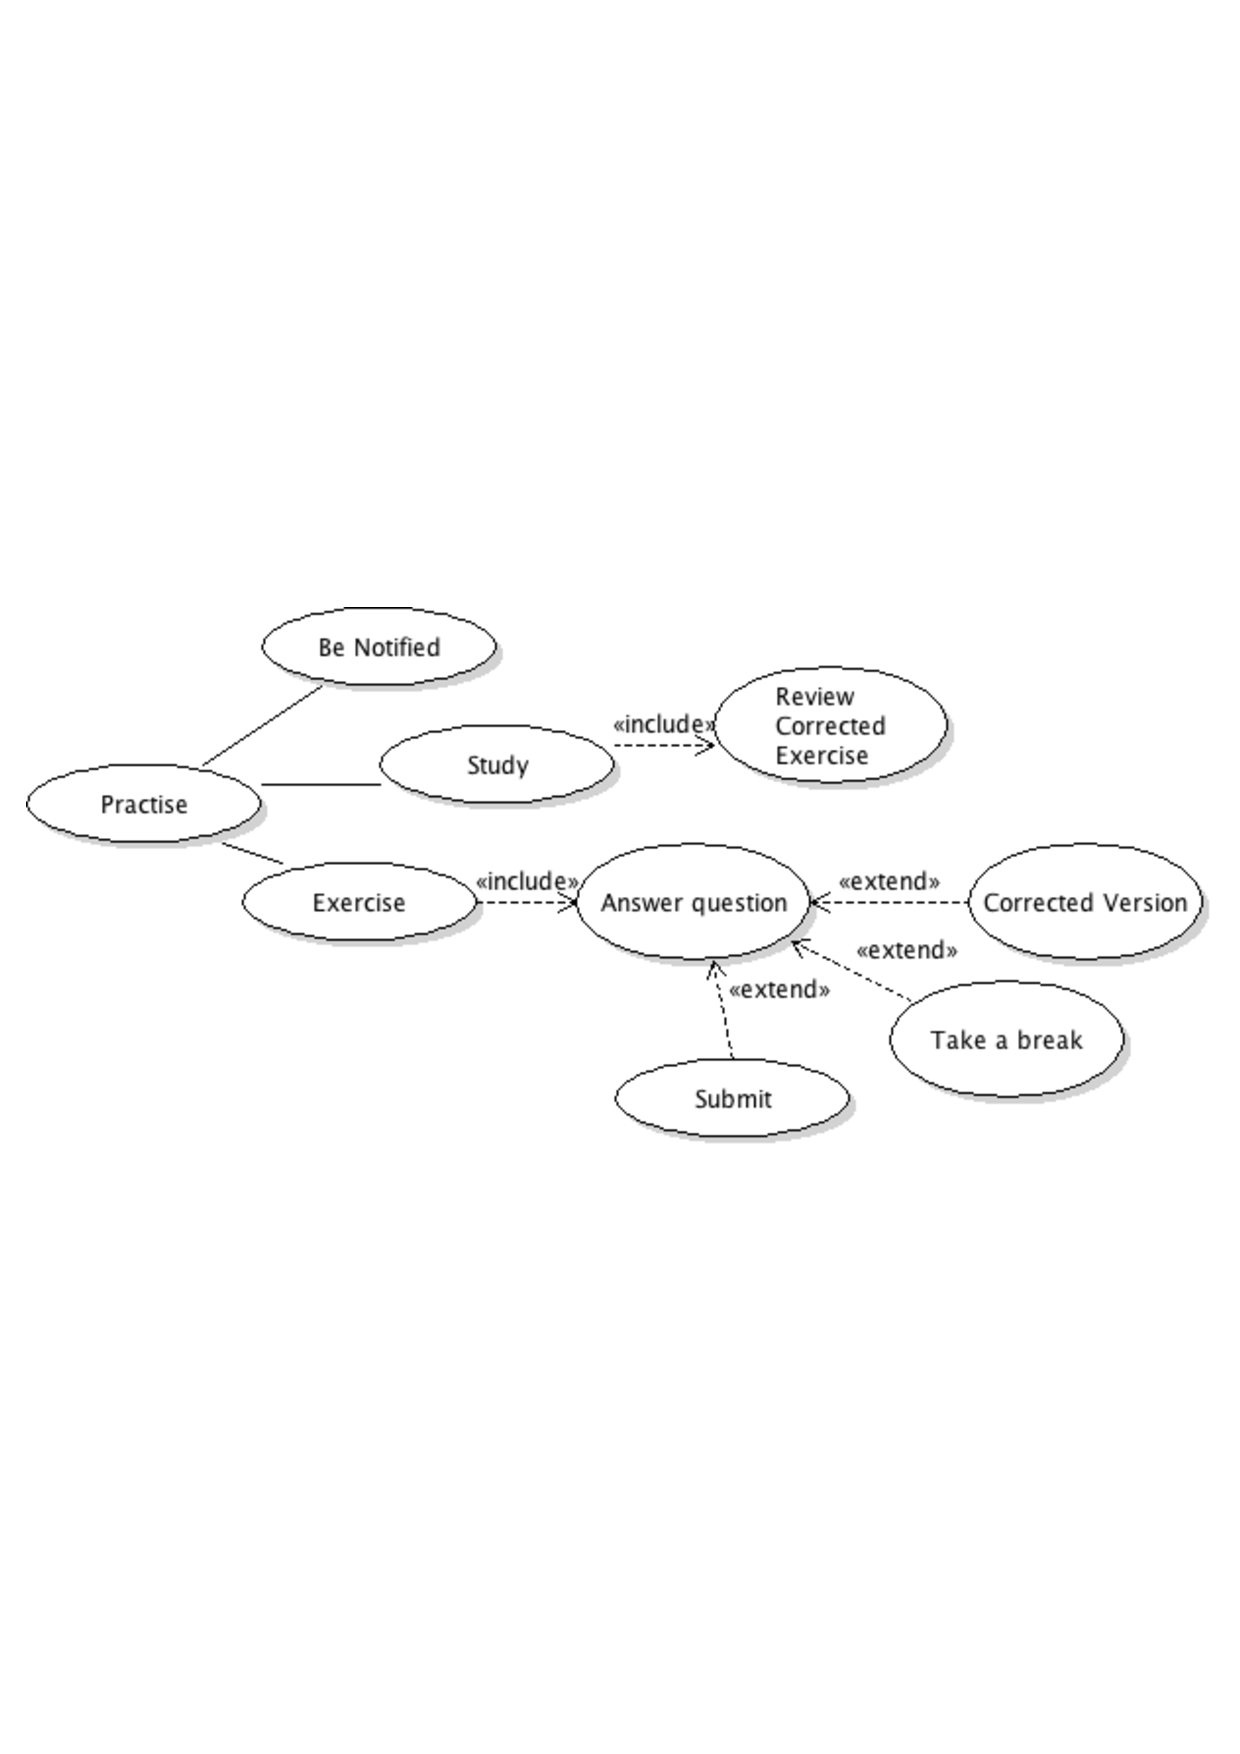
\includegraphics[width=\textwidth,  trim=2cm 10cm 2cm 11cm]{UML_figure/UC/student/UC_Student_Practise.pdf}
				\caption{Student Use Case : Practise}
			\end{center}
		\end{figure}
		A student exercises to improve himself. He/She answers questions.
	
	\subsection{Meditate}
	
	\begin{figure}[ht]
			\begin{center}
				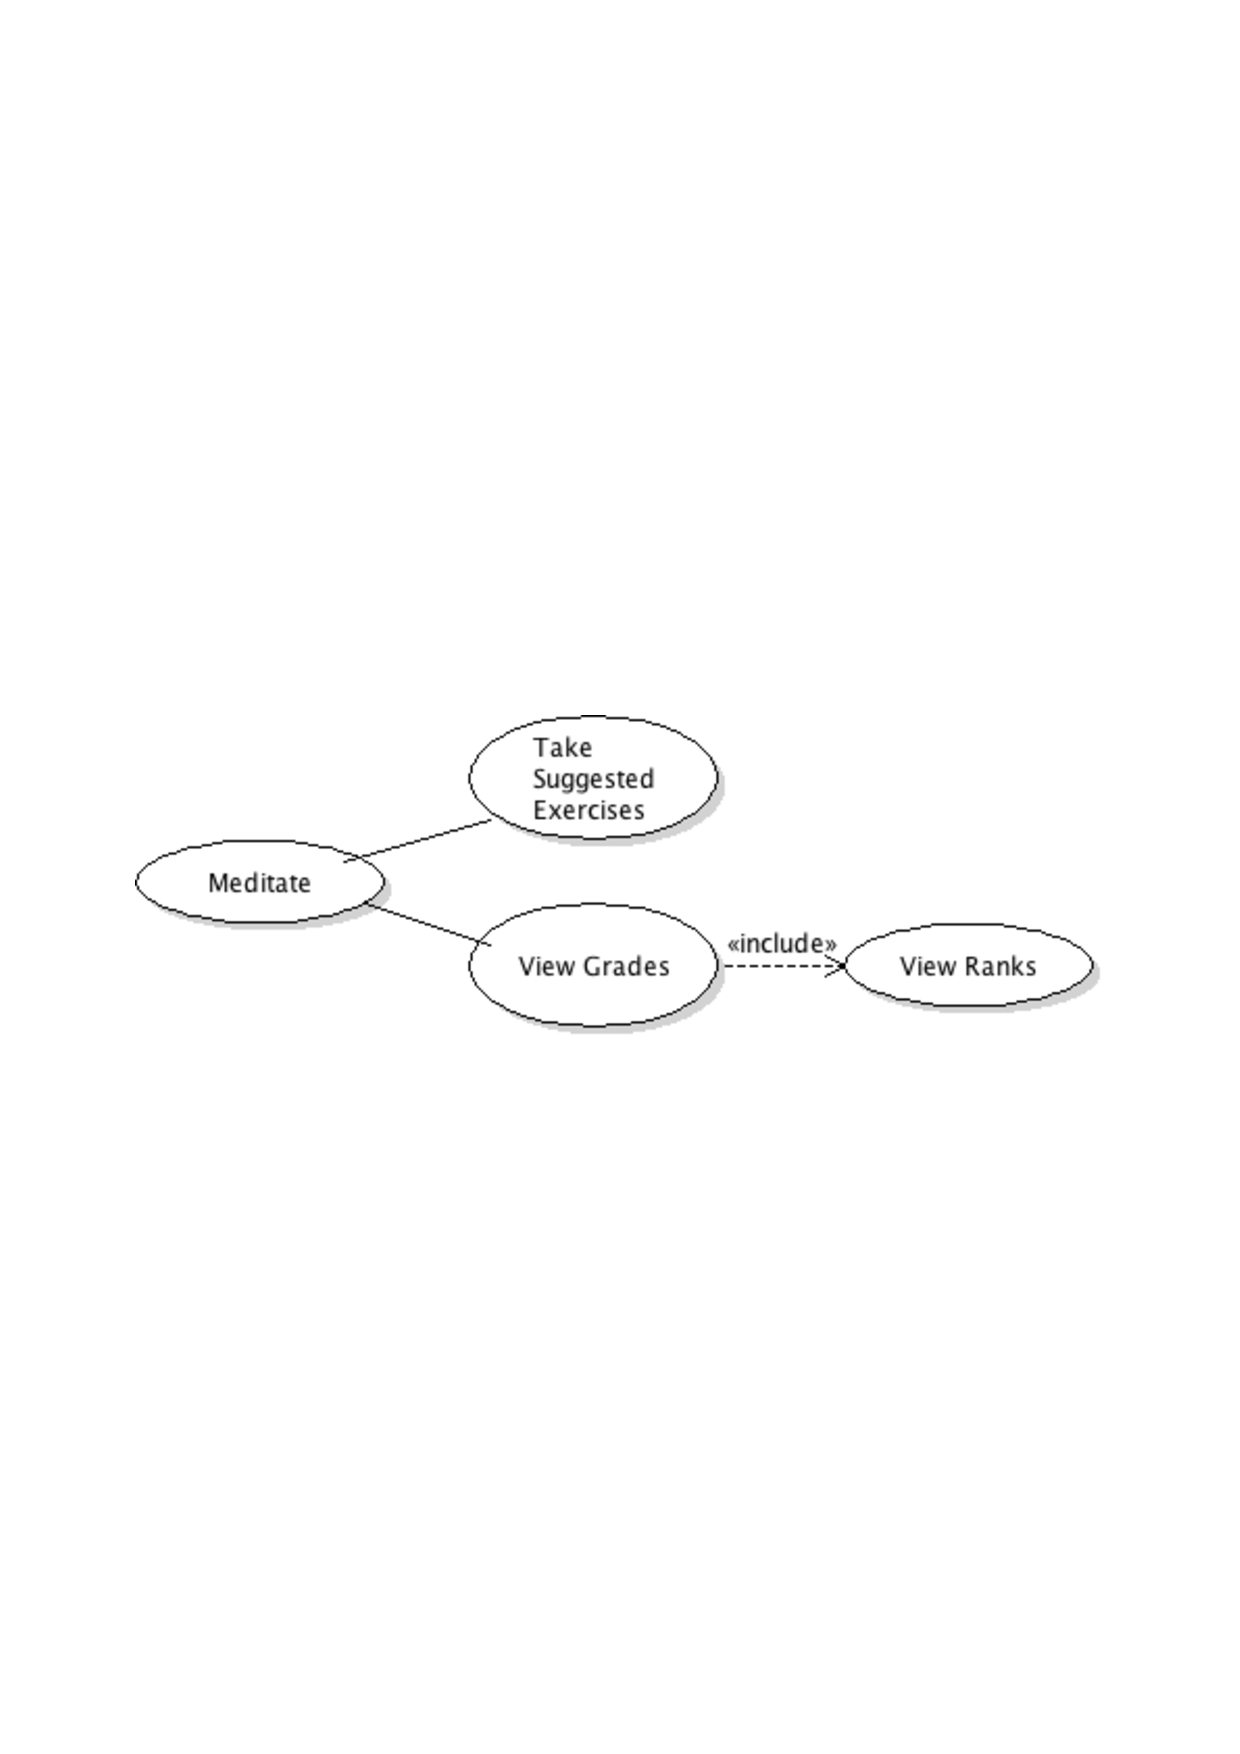
\includegraphics[width=\textwidth,  trim=2cm 10cm 2cm 11cm]{UML_figure/UC/student/UC_Student_Meditate.pdf}
				\caption{Student Use Case : Meditate}
			\end{center}
		\end{figure}
		\subsubsection{Suggested Exercises}
			The platform will provide exercises depending on student's weaknesses.
		\subsubsection{Grade}
			Student can see their grade for each exercises.
%end student section
\newpage
%begin teacher section
\section{Teacher}
	\subsection{General Use Case}
		\begin{figure}[ht]
			\begin{center}
				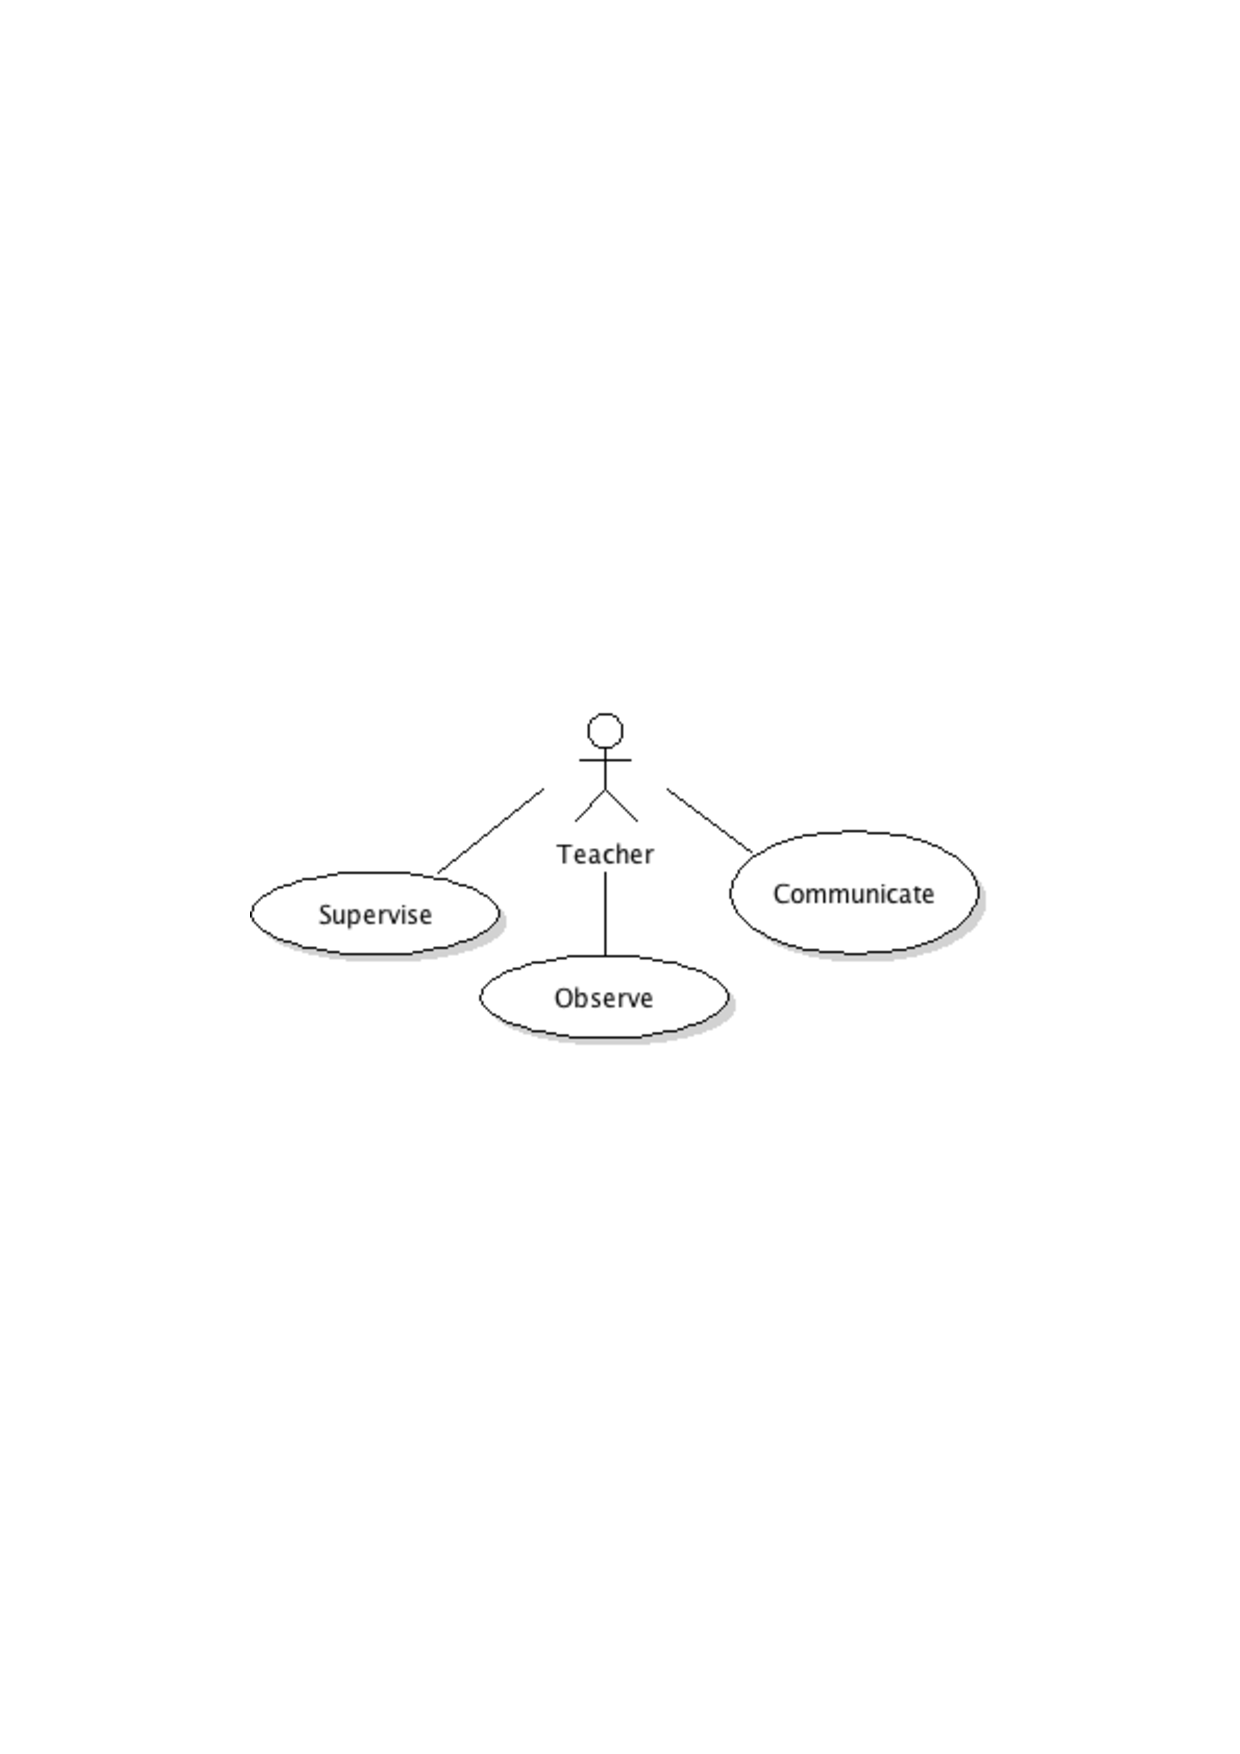
\includegraphics[width=\textwidth,  trim=2cm 10cm 2cm 11cm]{UML_figure/UC/teacher/UC_Teacher_General.pdf}
				\caption{Teacher Use Case : Overview}
			\end{center}
		\end{figure}
	\subsection{Supervise}
		A teacher writes exercises.
		\begin{figure}[ht]
			\begin{center}
				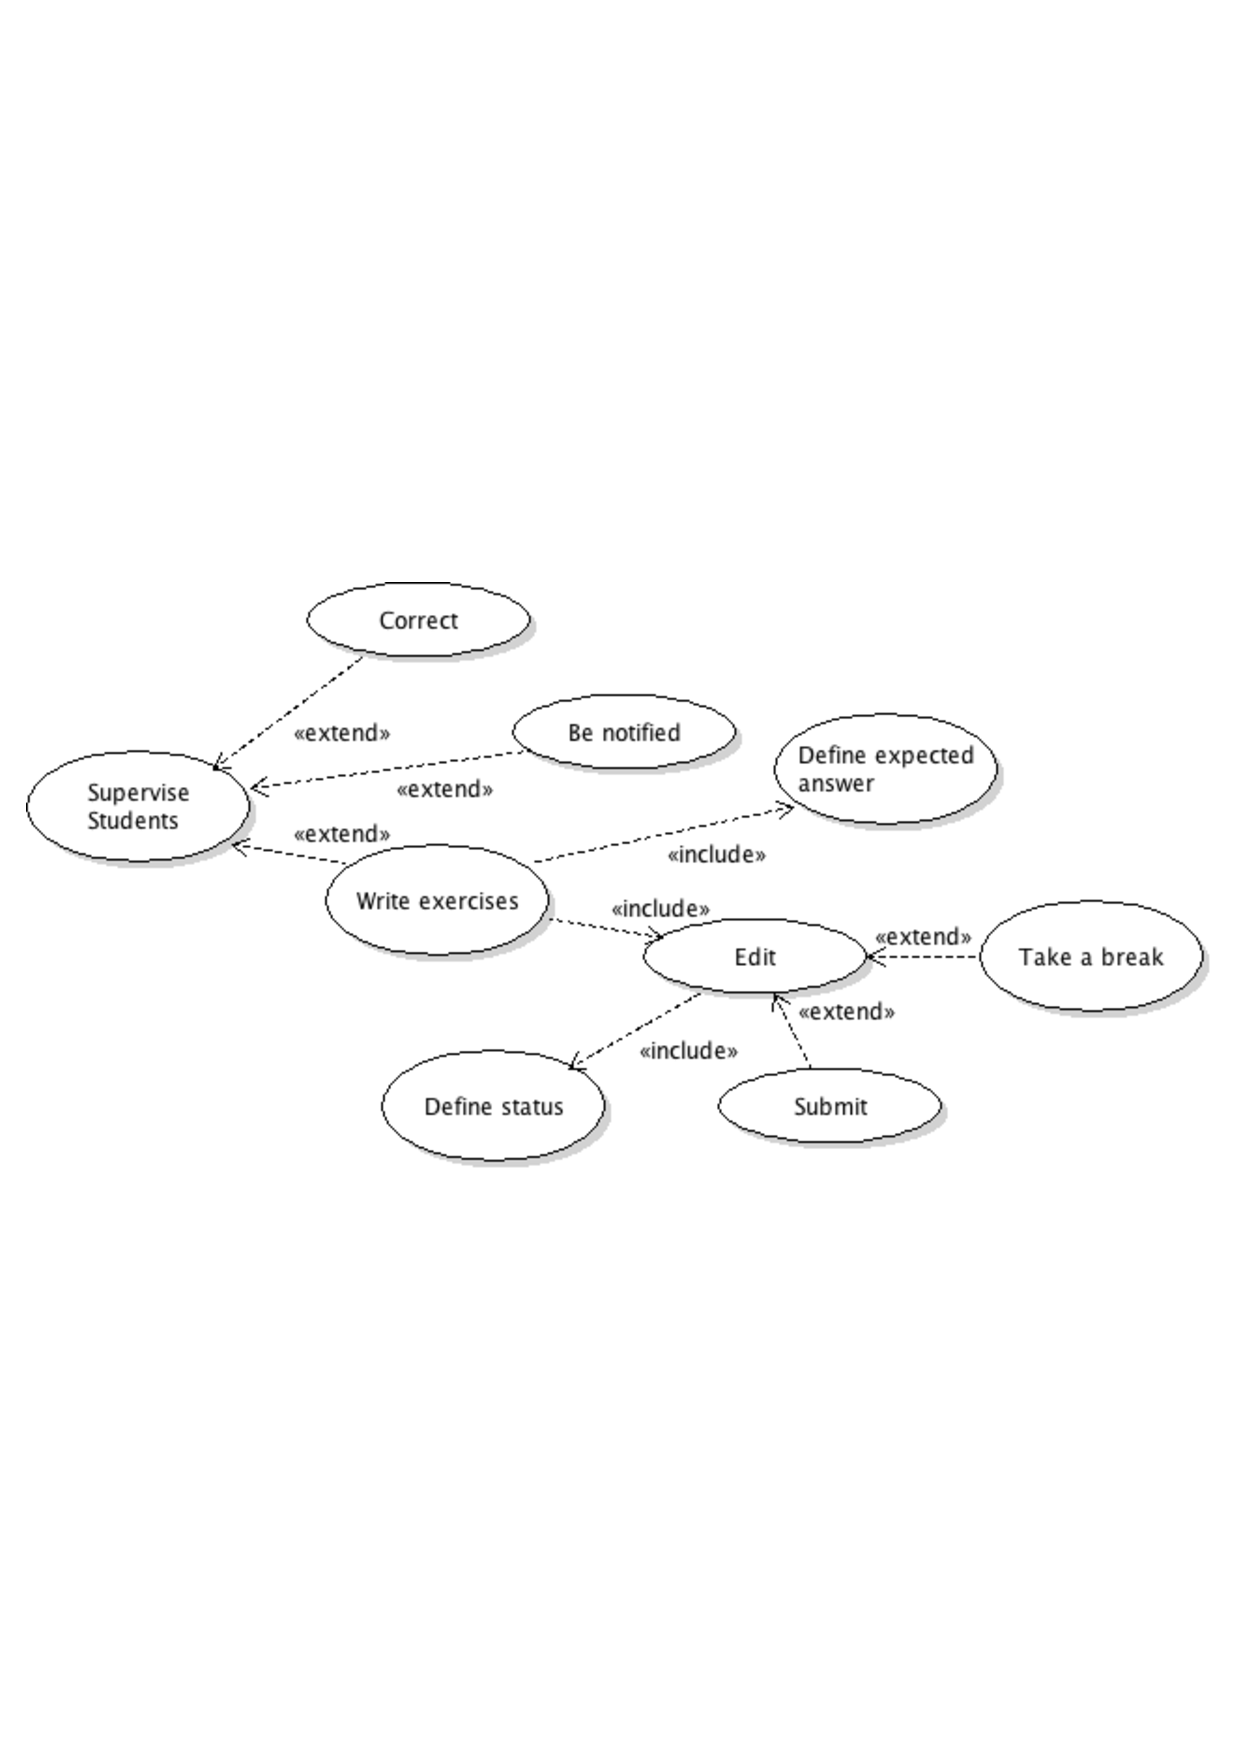
\includegraphics[width=\textwidth,  trim=2cm 10cm 2cm 9cm]{UML_figure/UC/teacher/UC_Teacher_Supervise.pdf}
				\caption{Teacher Use Case : Supervise}
			\end{center}
		\end{figure}
	\newpage
	\subsection{Observe}
		A teacher observes his students about how they get through on his/her exercise.
		\begin{figure}[ht]
			\begin{center}
				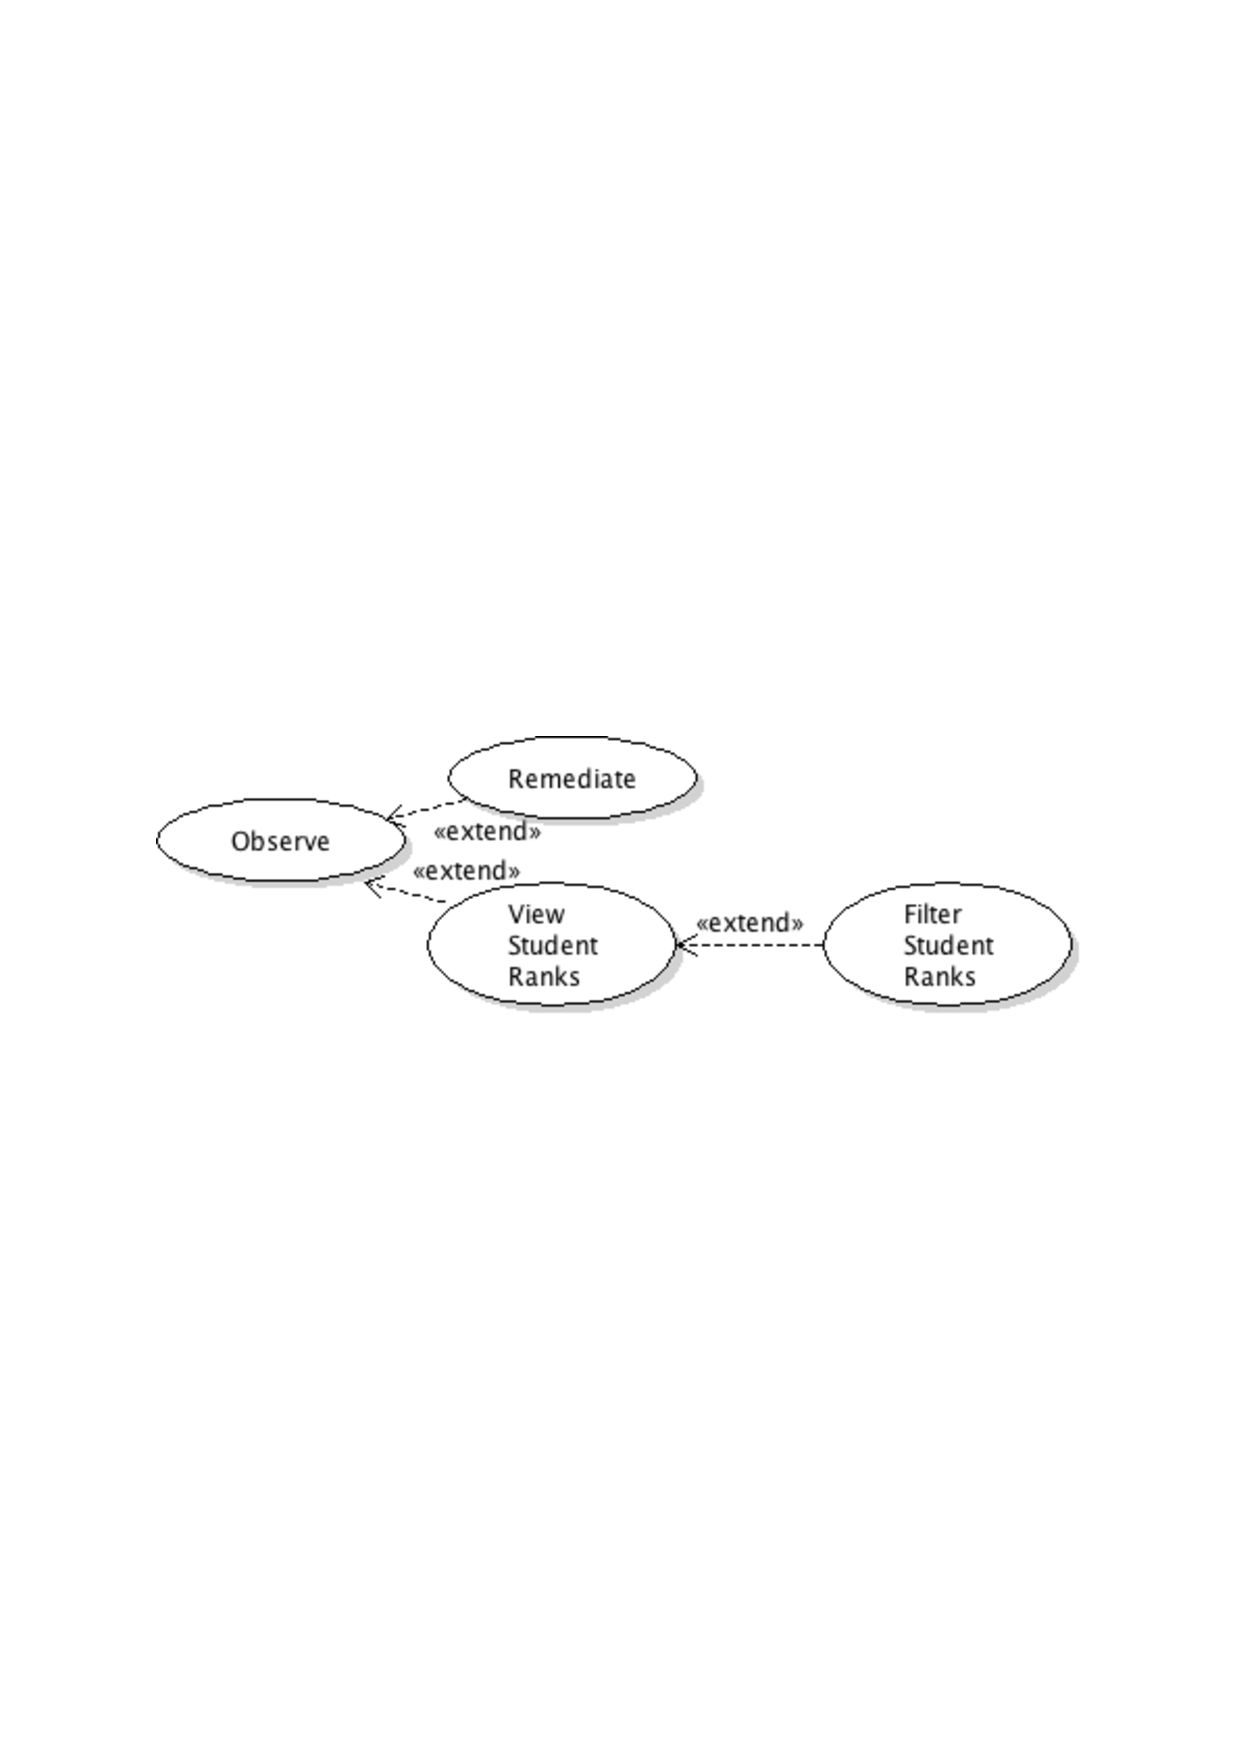
\includegraphics[width=\textwidth,  trim=2cm 10cm 2cm 11cm]{UML_figure/UC/teacher/UC_Teacher_Observe.pdf}
				\caption{Teacher Use Case : Observe}
			\end{center}
		\end{figure}
%end teacher section
\newpage
%begin administrator section
\section{Administrator}
	\subsection{General Use Case}
		\begin{figure}[ht]
			\begin{center}
				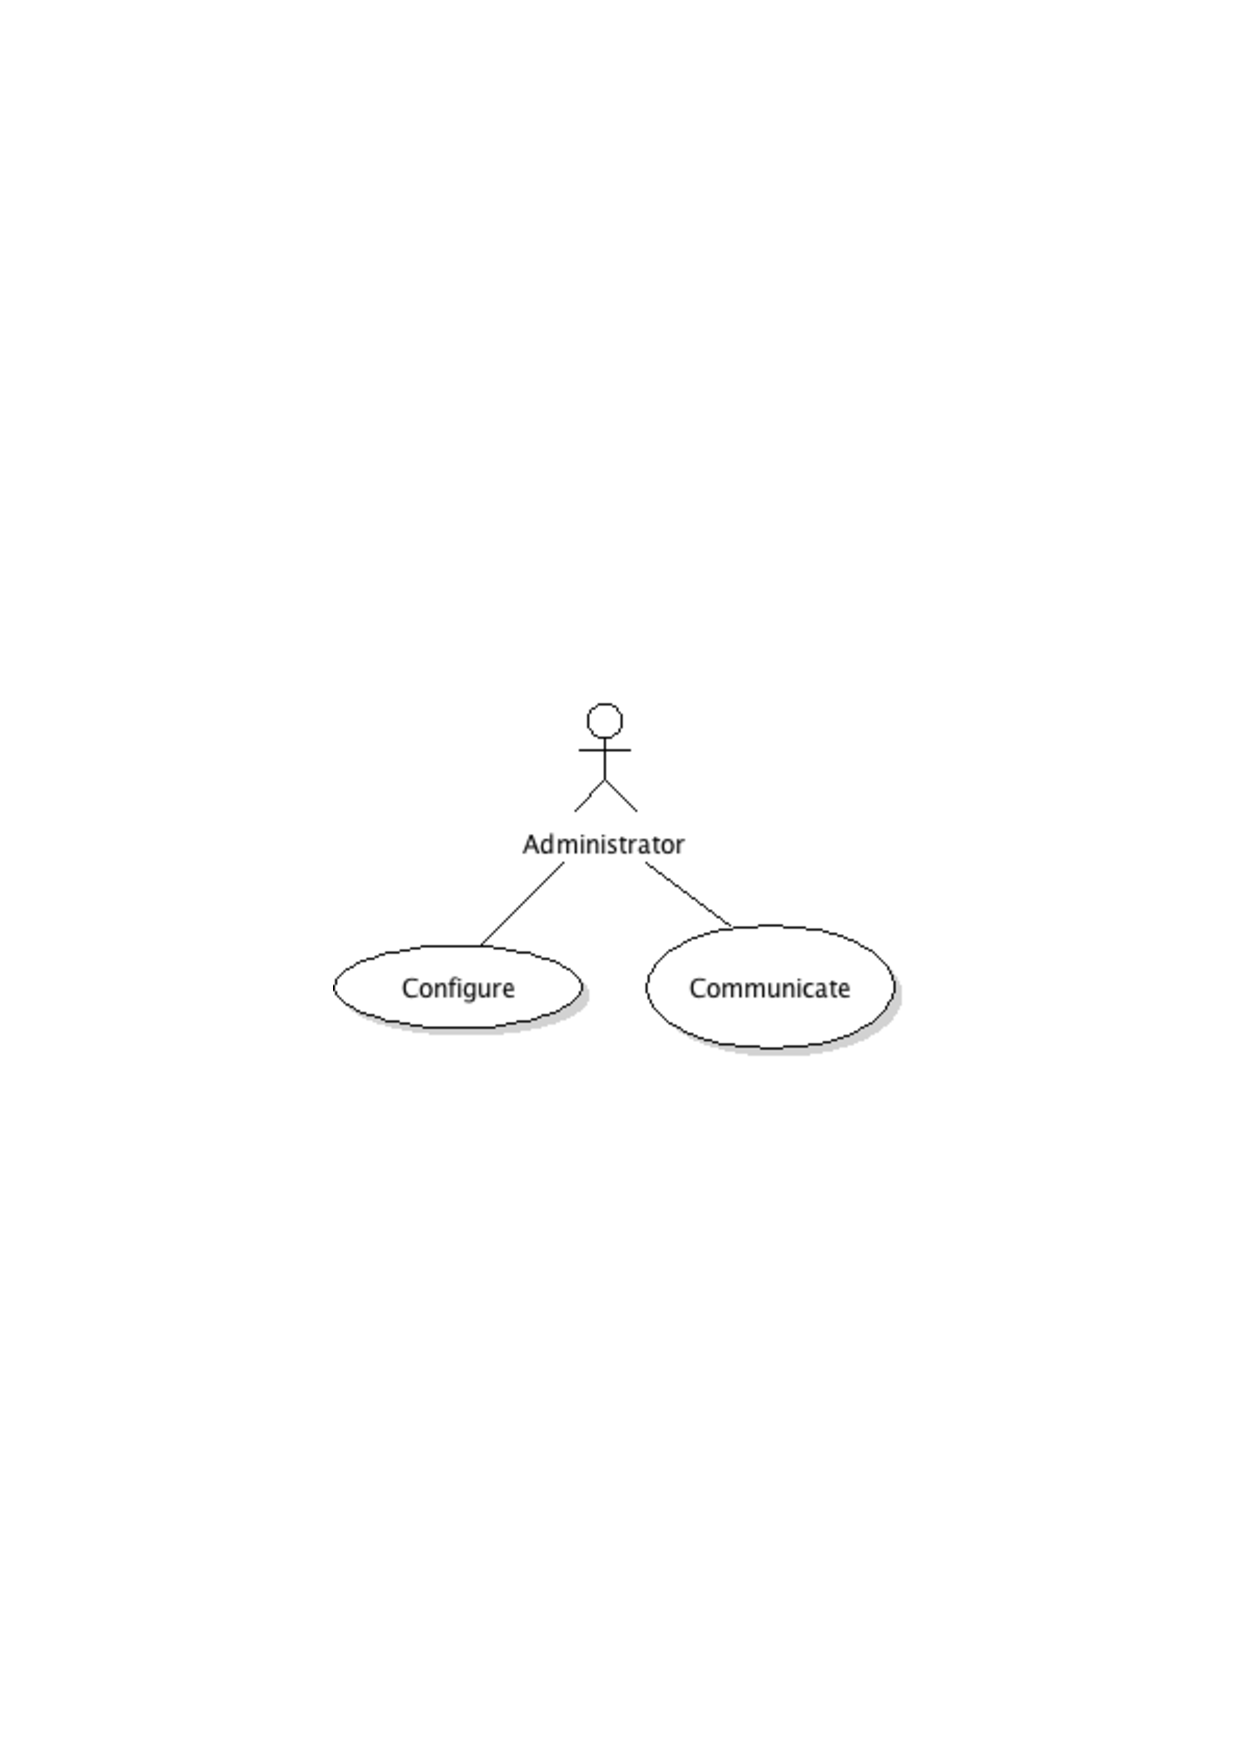
\includegraphics[width=\textwidth, trim=2cm 10cm 2cm 11cm]{UML_figure/UC/administrator/UC_Administrator_General.pdf}
				\caption{Administrator Use Case : Overview}
			\end{center}
		\end{figure}
	\subsection{Configure}
		The administrator task is to configure the platform.
%end administrator section
\newpage
%begin common user section
\section{Common registered user}
	\begin{figure}[ht]
		\begin{center}
			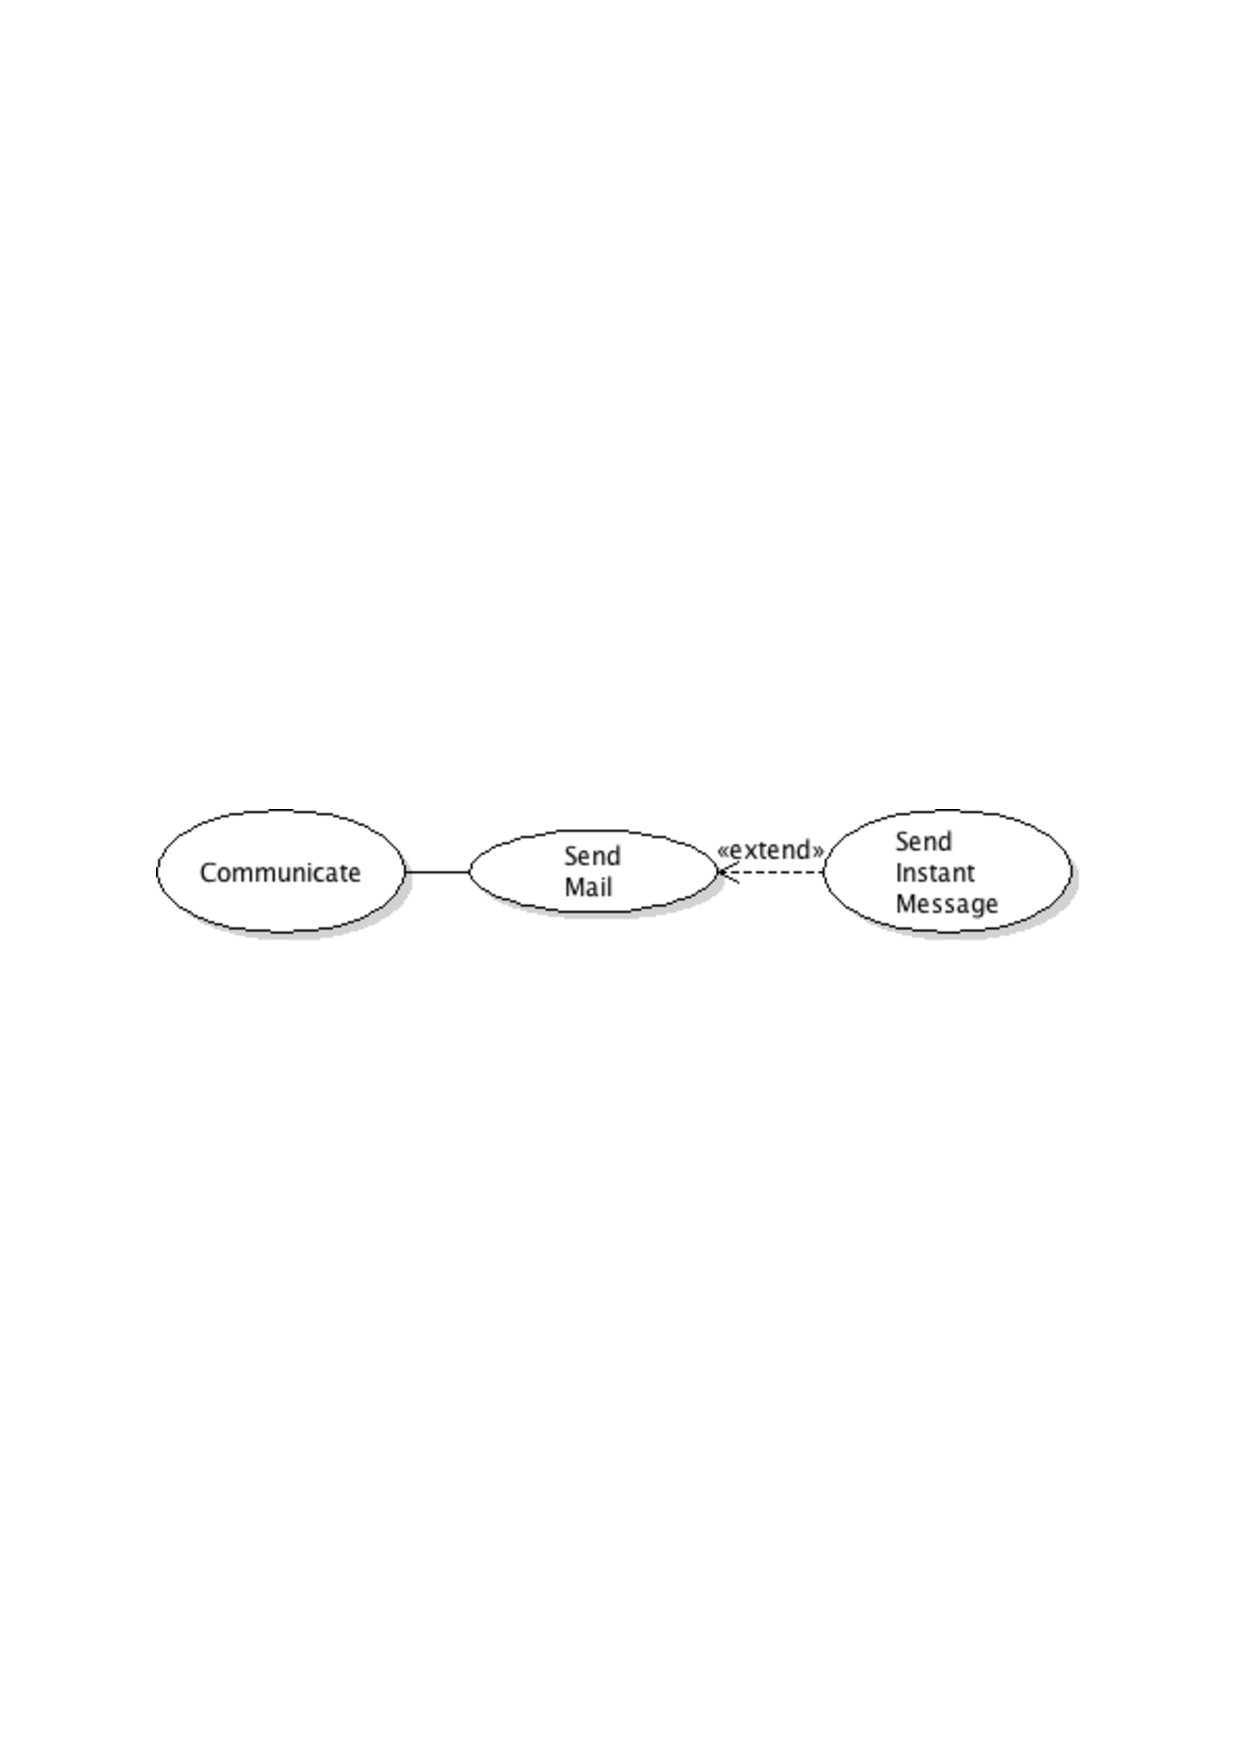
\includegraphics[width=\textwidth,  trim=2cm 10cm 2cm 11cm]{UML_figure/UC/common/UC_Common_Communicate.pdf}
			\caption{Registered user Use Case : Communicate}
		\end{center}
	\end{figure}
	\subsection{Communicate}
		Registered user can communicate each other.
	\subsection{Send Mail}
		Communication provide by mail exchange.
	\subsection{Send Instant Message}
		Communication provide by instant message exchange.
%end common user section













